%!TEX root = JakubJedryszek2014.tex

\cleardoublepage


\chapter{Background}
\label{background}

This chapter is a brief introduction of all technologies and tools used in this thesis. They are: AADL modeling language, BLESS (AADL annex language), SPARK Ada programming language and its verification tools. There is also an overview of the context in which this work has been done: Integrated Clinical Environment (ICE) standard and PCA pump (ICE compliant device). This is followed by main topic of the thesis: code generation from AADL and analysis of existing AADL translators (Ocarina, RAMSES).



\section{Integrated Clinical Environment}
\label{background:ice}
%http://santos.cis.ksu.edu/MDCF/doc/ICE-Motivation.pdf

The concept of the "Integrated Clinical Environment" (ICE) was initiated and championed by Dr. Julian Goldman from Center for Integration of Medicine \& Innovative Technology.\footnote{http://www.cimit.org/} The main idea is to create a platform for integrating medical devices in a local area network. ICE will enable clinicians and software system to make decisions based not only on output from one device, but from different devices working together in network. Moreover, ICE comprises components that may be implemented by different vendors. Such components are medical devices and applications to supervise them. The purpose of ICE is to solve current issues with medical devices, which usually operate independently and requires more human attention and control through checking output of every device manually and then making decisions. ICE propose a concept of Medical Application Platform \cite{MedicalApplicationPlatforms:Paper} that assure medical devices interoperability and provides execution environment for clinical applications. Different devices can exchange data and centralized system can make decisions (based on this data) automatically. For example when PCA pump infuse some drug to patient's vein and Pulse Oximeter detects low oxygen level, ICE can coordinate PCA pump shutdown. 

Figure \ref{figure:ice} presents high-level overview of one particular application of an ICE system. Medical devices (PCA Pump, Respiratory Rate Monitor and Pulse Oximeter) are connected to the system, which monitors or controls them. There is communication between devices and ICE in order to exchange data. ICE can make decisions (such as PCA Pump shutdown) based on them.

\begin{figure}[ht]%t=top, b=bottom, h=here
    \begin{center}
    	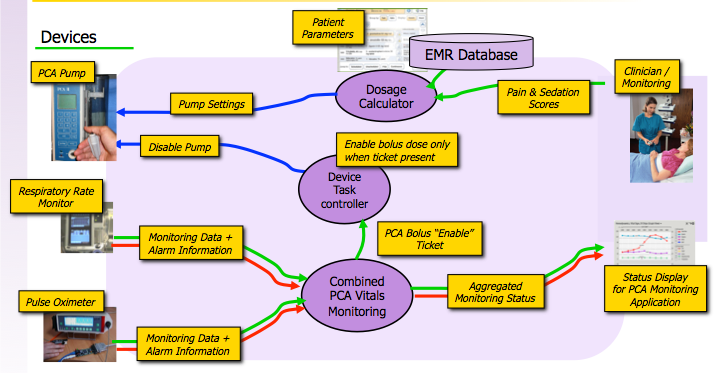
\includegraphics[height=3.5in]{figures/ice.png}   	
    \end{center}
    \caption{ICE Closed Loop Control}
    \label{figure:ice}
\end{figure}


\section{Medical Device Coordination Framework}
\label{background:mdcf}
%http://santos.cis.ksu.edu/MDCF/doc/MDCF-Tutorial-Overview.pdf

Medical Device Coordination Framework (MDCF) \cite{MedicalApplicationPlatforms:Paper}, jointly developed by SAnToS Laboratory (Kansas State University) and University of Pennsylvania is prototype implementation of ICE. It is an open, experimental platform to bring together academic researchers, industry vendors, and government regulators. This project is a response to a request from Food and Drug Administration (FDA) to build a prototype of ICE. There is a vision of different medical devices, created by different vendors, connected and working under centralized system. MDCF is designed to illustrate by example issues related to functional concepts, safety, security, verification and certification. 

The following comprise the goals of the MDCF project:
\begin{itemize}
	\item Open source infrastructure
	\item Meet performance requirements of realistic clinical scenarios
	\item Provide middleware with reliability, real-time, security
	\item Provide an effective app programming model and development environment with integrated verification/validation support and construction of regulatory artifacts
	\item Support evaluation of device interfacing concepts
	\item Illustrate how to support real and mock devices
	\item Illustrate envisioned regulatory oversight and 3rd party certification
\end{itemize}

Currently, MDCF use only mock devices, which are Java desktop applications. PCA Pump Prototype, developed in this thesis, aims to be the realistic hardware device targeted specifically for the MDCF.

MDCF uses a publish-subscribe architecture for communication between components: apps and devices. Figure \ref{figure:mdcf} presents MDCF structure. Devices, such as PCA pump, are connected to Message Bus, which along with Device Manager and Device Database ensures communication with Application Manager \cite{MedicalApplicationPlatforms:Paper}.

\begin{figure}[ht]%t=top, b=bottom, h=here
    \begin{center}
    	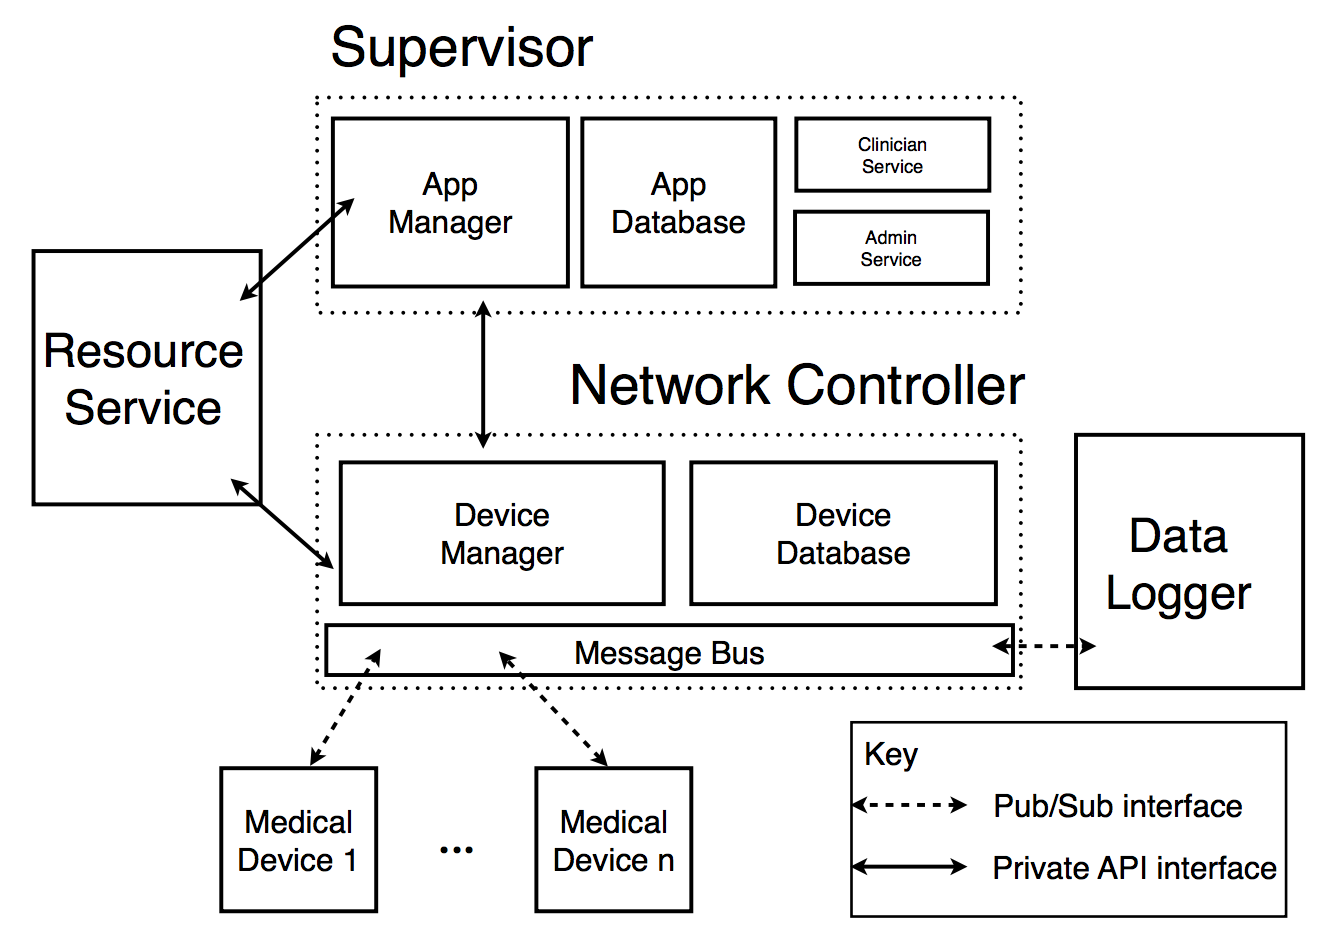
\includegraphics[width=0.9\textwidth]{figures/mdcf.png}    	
    \end{center}
    \caption{MDCF architecture and example app virtual machine (lower right)}
    \label{figure:mdcf}
\end{figure}



\section{AADL}
\label{background:aadl}

AADL stands for Architecture Analysis \& Design Language. It is used to model embedded and real-time systems. AADL allows for description of both software and hardware parts of a system. It can be used not only for design phase of software development process, but also for analysis, verification, and code generation.

AADL has its roots in DARPA\footnote{http://www.darpa.mil} funded research. The first version (1.0) was approved in 2004 under technical leadership of Peter Feiler.\footnote{http://wiki.sei.cmu.edu/aadl/index.php/The\_Story\_of\_AADL/} AADL is develop by SAE AADL standard committee.\footnote{https://wiki.sei.cmu.edu/aadl/index.php/Main\_Page} AADL version 2.0 was published in January 2009. The most recent version (2.1) was published in September 2012.\footnote{https://wiki.sei.cmu.edu/aadl/index.php/Standardization}

AADL is a language for Model-Based Engineering \cite{AadlBook}. It can be represented in textual and graphical form. There are tools, like plug-in for OSATE (see Section \ref{background:aadl:osate}) that enable transformation of textual representation into graphical or XML. 

\begin{wrapfigure}{r}{0.3\textwidth}
  \begin{center}
    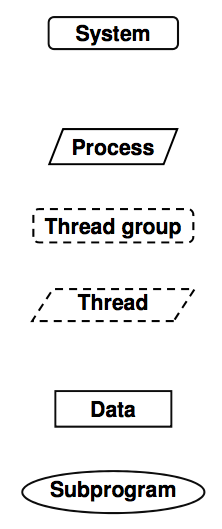
\includegraphics[width=0.25\textwidth]{figures/aadl-app-components.png}
  \end{center}
  \caption{AADL Application Software Components}
  \label{figure:aadl_app_software_components}
\end{wrapfigure}

AADL contains entities for modeling software and hardware components, and allows to create interactions and dependencies between them.

AADL Execution Platform Components and Devices:
\begin{itemize} \itemsep1pt \parskip0pt \parsep0pt
	\item Processor / Virtual Processor - Provides thread scheduling and execution services
	\item Memory - provides storage for data and source code
	\item Bus / Virtual Bus - provides physical/logical connectivity between execution platform components
	\item Device - interface to external environment
\end{itemize}

Application Software Components of AADL (Figure \ref{figure:aadl_app_software_components}):
\begin{itemize} \itemsep1pt \parskip0pt \parsep0pt
	\item System - hierarchical organization of components
	\item Process - protected address space
	\item Thread group - logical organization of threads
	\item Thread - a schedulable unit of concurrent execution
	\item Data - potentially sharable data
	\item Subprogram - callable unit of sequential code
\end{itemize}

\singlespacing
\begin{figure}[ht]%t=top, b=bottom, h=here
    \begin{center}
    	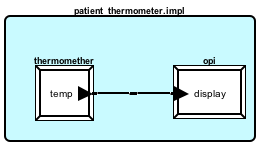
\includegraphics[width=0.4\textwidth]{figures/patient_thermometer.png}    	
    \end{center}
    \caption{AADL model of simple thermometer}
    \label{figure:patient_thermometer}
\end{figure}
\doublespacing 

An example AADL model is shown in graphical representation, in the Figure \ref{figure:patient_thermometer}. Its textual representation is presented in the Figure \ref{listing:patient_thermometer}.

\begin{figure}[ht]
\singlespacing
\begin{lstlisting}[language=aadl, frame=single, gobble=0]
package Thermometer
public 
with Base_Types;

	system patient_thermometer
	end patient_thermometer;
	system implementation patient_thermometer.impl
	subcomponents
		thermomether : device thermometer_device.impl;
		opi : device operator_interface.impl;
	connections
		tdn : port thermomether.temp -> opi.display;
	end patient_thermometer.impl;

	device operator_interface
	features
		display : in data port Base_Types::Integer;
	end operator_interface;
	device implementation operator_interface.impl
	end operator_interface.impl;

	device thermometer_device
	features
		temp : out data port Base_Types::Integer;
	end thermometer_device;
	device implementation thermometer_device.impl
	end thermometer_device.impl;
end Thermometer;
\end{lstlisting} 
\doublespacing
\caption{AADL model of simple thermometer}
\label{listing:patient_thermometer}
\end{figure}
%another example: https://wiki.sei.cmu.edu/aadl/images/7/73/AADLV2Overview-AADLUserDay-Feb_2010.pdf (slide 16)

There are several tools for AADL model support, such as: OSATE (see Section \ref{background:aadl:osate}), STOOD (AADL design tool),\footnote{http://www.ellidiss.com/products/stood} ADELE (graphical editor),\footnote{https://wiki.sei.cmu.edu/aadl/index.php/Adele} Cheddar (real time scheduling tool),\footnote{http://beru.univ-brest.fr/~singhoff/cheddar} AADLInspector (model processing framework),\footnote{http://www.ellidiss.com/products/aadl-inspector} or Ocarina (see Section \ref{background:codegen:ocarina}).

AADL focuses on architectural modeling, but it can be extended via the following methods:
\begin{itemize}
	\item user-defined properties: user can extend the set of applicable properties and add their own to specify their own requirements
	\item {language annexes (the core language is enhanced by annex languages that enrich the architecture description. For now, the following annexes have been defined):
		\begin{itemize}
			\item Behavior annex: add components behavior with state machines (e.g. BLESS, see Section \ref{background:bless})
			\item Error-model annex: specifies fault and propagation concerns
			\item ARINC653 annex: defines modeling patterns for modeling avionics systems
			\item Data-Model annex: describes the modeling of specific data types and structures with AADL
		\end{itemize}
		}
\end{itemize}

More details about AADL can be found in Peter Feiler's book "Model-Based Engineering with AADL" \cite{AadlBook}.

AADL is used as a modeling language in this thesis.


\subsection{OSATE}
\label{background:aadl:osate}

Open Source AADL Tool Environment (OSATE) is a set of plug-ins on top of the Eclipse platform. It provides a tool set for front-end processing of AADL models. OSATE is developed mainly by SEI (Software Engineering Institute - Carnegie Mellon University).\footnote{http://www.aadl.info/aadl/currentsite/tool/osate.html} The latest available version of OSATE at the time when this thesis was published is OSATE2.\footnote{https://wiki.sei.cmu.edu/aadl/index.php/Osate\_2} 

OSATE relies on EMF,\footnote{http://www.eclipse.org/modeling/emf/} UML2 and Xtext.\footnote{http://www.eclipse.org/Xtext/} It comprises, e.g., an AADL project wizard, AADL Navigator, and AADL syntax analyzer. OSATE enables the conversion of AADL in textual representation into its standardized graphical representation. There are also plug-ins for OSATE, such as the BLESS\footnote{http://bless.santoslab.org/node/5} and OCARINA\footnote{http://libre.adacore.com/tools/ocarina/} plug-ins.

OSATE has been used to develop AADL models for this thesis and work with already existing models.



\section{BLESS}
\label{background:bless}
BLESS (Behavior Language for Embedded Systems with Software) is AADL annex sub-language defining behavior of components for AADL \cite{Bless:Paper}. BLESS comes with a verification framework that enables a developer to build proofs of AADL models of embedded electronic systems with software.

BLESS annex subclauses can be added to AADL models transparently without interfering with other uses of AADL. It includes a verification-condition (VC) generation framework and an accompanying proof tool that enables engineers to prove VCs via proof scripts build from system axioms and rules from a user-customizable rule library \cite{Bless:Paper}.

BLESS contains three AADL annex sub-languages:
\begin{itemize} \itemsep1pt \parskip0pt \parsep0pt
	\item Assertion - assertions can be attached individually to AADL features (e.g. ports)
	\item subBLESS - can be attached only to subprograms; it has only value transformations and Assertions without time expressions
	\item BLESS - it can be attached to AADL thread, device or system components; it contains states, transitions, timeouts, actions, events and Assertions with time expressions
\end{itemize}

The BLESS tool framework is implemented as a publicly available open source plug-in for OSATE (mentioned in Section \ref{background:aadl:osate}). It includes an editor for BLESS specifications and an environment operating the BLESS proof engine \cite{Bless:Paper}.

In the work for this thesis, subset of BLESS is translated into SPARK contracts and assertions. Detailed overview of supported features can be found in Section \ref{codegen:mapping:bless}.



\section{SPARK Ada}
\label{background:spark}

%http://www.cs.swan.ac.uk/~csetzer/lectures/critsys/09/critsysfinal2.pdf

The Ada programming language was originally designed to meet the US Department of Defense Requirements for programming military applications. Since its first version (Ada 83) it has evolved through multiple versions: Ada 95, Ada 2005 and Ada 2012 (released in December 10, 2012).\footnote{http://www.ada2012.org} Ada is actively used in many real-world projects in critical application domains,\footnote{http://www.seas.gwu.edu/\textasciitilde{}mfeldman/ada-project-summary.html} e.g. Aviation (Boeing\footnote{http://archive.adaic.com/projects/atwork/boeing.html}), Railway Transportation, Commercial Rockets, Satellites and even Banking. One of the main goals of Ada is to ensure software correctness and safety. Ada includes features that eliminate common errors involving pointers, array bounds violations and unprincipled control flow, in comparison to other programming languages (see Figure \ref{figure:developer-responsibility-in-ada}). This is achieved not only by language capabilities, but also by tools for testing and verification. 

SPARK is a programming language and static verification technology designed specifically for the development of high integrity software. It is a "safe" subset of Ada, designed to be amenable to state analysis and formal methods, by collection of analysis and verification tools. Some Ada constructs are excluded from SPARK to make static analysis feasible \cite{Spark:Article}. SPARK 2005 does not include constructs such as pointers, dynamic memory allocation or recursion \cite{Spark:Article}. Verification tools (see Section \ref{background:sparkverification}) produce Verification Conditions (VCs) to check program correctness. Sample Verification Condition contains checks for:
\begin{itemize} %\itemsep1pt \parskip0pt \parsep0pt
    \item array index out of range
    \item type range violation
    \item division by zero
    \item numerical overflow
\end{itemize}

\begin{figure}[h]%t=top, b=bottom, h=here
    \begin{center}
    	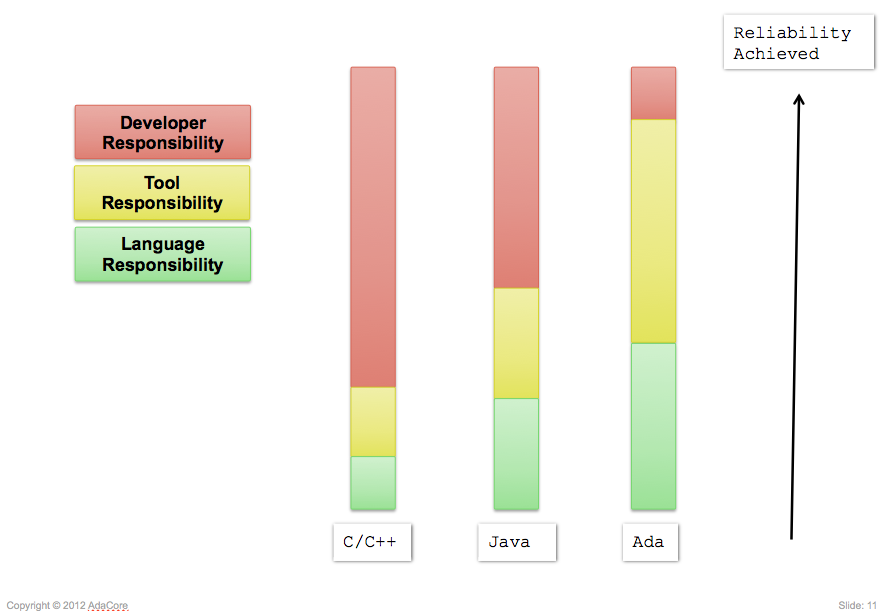
\includegraphics[width=0.9\textwidth]{figures/developer_responsibility_in_ada.png}    	
    \end{center}
    \caption{Developer responsibility in Ada.\protect\footnotemark }
    \label{figure:developer-responsibility-in-ada}
\end{figure}
\footnotetext{http://www.slideshare.net/AdaCore/ada-2012}

SPARK is used not only for research, but also in industry: aerospace (e.g., EuroFighter Typhoon aircraft,\footnote{http://www.eurofighter.com/} The Lockheed Martin C130J\footnote{http://www.lockheedmartin.com/us/products/c130/c-130j-variants/c-130j-30.html} and standard DO-178B\footnote{http://www.adacore.com/gnatpro-safety-critical/avionics/do178b/}), security (e.g., MULTi-application Operating System\footnote{http://www.cardwerk.com/smartcards/MULTOS/}), air traffic management (e.g., iFACTS system\footnote{http://www.adacore.com/customers/uks-next-generation-atc-system/}) \cite{Barnes:Book}. In practice, because the features of SPARK are limited and because the use of SPARK can be labor intensive, the embedded critical components are written in SPARK while the non-critical components are written in Ada \cite{Spark:IndustrialExp}.

First version of SPARK was based on Ada 83. The second version (SPARK 95) - on Ada 95. SPARK 2005 is based on Ada 2005. It is a subset of Ada 2005 with annotations. The annotation language support flow analysis and formal verification. Annotations are encoded in Ada comments (via the prefix \lstinline{--#}). This approach allows every SPARK 2005 program to be a valid Ada 2005 program. SPARK annotations contains code contracts (see Table \ref{table:SparkAnnotations}), which are analyzed by verification tools, but ignored by Ada compiler.

\begin{figure}[ht]
\singlespacing
\begin{lstlisting}[language=ada, frame=single, gobble=0]
procedure Increment (X : in out Integer);
--# derives X from X;
--# pre X < Integer'Last;
--# post X = X~ + 1;
\end{lstlisting} 
\doublespacing
\caption{Sample SPARK procedure with code contracts}
\label{listing:SPARK2005Contracts}
\end{figure}

Figure \ref{listing:SPARK2005Contracts} presents simple procedure with code contracts. It increments variable given as parameter by 1. The \lstinline{derives} clause specify variable dependency. Its future value depends on its current value. There is precondition saying that the value has to be lower than maximum value of \lstinline{Integer} type, to avoid overflow. There is also post condition, which states that the value of variable (given as parameter) after the procedure execution has to be equal to its previous value incremented by 1 ('\lstinline{~}' attached to variable means value of this variable, before procedure execution).

SPARK 2014\footnote{http://www.spark-2014.org} (based on Ada 2012) is under development. There is partial tool support (in GNAT Programming Studio), but some language features (such as tasking) are still not supported. Ada 2012 contains code contracts, which was inspired by previous versions of SPARK. Thus SPARK 2014 is just a subset of Ada 2012 \cite{Spark2014:Paper}. Some of Ada 2012 features are not allowed in SPARK, e.g.:
\begin{itemize} %\itemsep1pt \parskip0pt \parsep0pt
 	\item Access types (pointers)
 	\item Exceptions
	\item Aliasing between variables
	\item The goto statement
	\item Concurrency features of Ada (Tasking) - it's part of SPARK 2014 road-map to include support for tasking in the future, although likely not this year
	\item Side effects in expressions and functions
\end{itemize}

Table \ref{table:SparkAnnotations} presents fundamental SPARK 2005 annotations and their equivalents in SPARK 2014 (Ada 2012).

\singlespacing
\begin{center}
	\begin{longtable}{| p{1.3in} | p{1.3in} | p{3.4in} |}
		\caption{Fundamental SPARK annotations}
		\label{table:SparkAnnotations}
		\\
		\hline
		\multicolumn{1}{|c|}{\textbf{SPARK 2005}} & \multicolumn{1}{|c|}{\textbf{SPARK 2014}} & \multicolumn{1}{|c|}{\textbf{Description}} \\ \hline
		\endfirsthead

		\multicolumn{3}{c}%
		{{\bfseries \tablename\ \thetable{} -- continued from previous page}} \\
		\hline 
		\multicolumn{1}{|c|}{\textbf{SPARK 2005}} & \multicolumn{1}{|c|}{\textbf{SPARK 2014}} & \multicolumn{1}{|c|}{\textbf{Description}} \\ \hline
		\endhead

		\hline \multicolumn{3}{|r|}{{Continued on next page}} \\ \hline
		\endfoot

		\hline %\hline
		\endlastfoot

		\begin{lstlisting}
			--# global
		\end{lstlisting} 
		& 
		\begin{lstlisting}[language=ada2012]
			Global
		\end{lstlisting} 
		& 
		list of used global variables within subprogram 

		\\ \hline

		\begin{lstlisting}
			--# derives
		\end{lstlisting} 
		& 
		\begin{lstlisting}[language=ada2012]
			Depends
		\end{lstlisting} 
		& 
		describe dependencies between variables

		\\ \hline

		\begin{lstlisting}
			--# own 
		\end{lstlisting} 
		& 
		\begin{lstlisting}[language=ada2012]
			Abstract_State
		\end{lstlisting} 
		& 
		declare variables defined in package body

		\\ \hline

		\begin{lstlisting}
			--# initializes
		\end{lstlisting} 
		& 
		\begin{lstlisting}[language=ada2012]
			initializes
		\end{lstlisting} 
		& 
		indicates variables, which are initialized

		\\ \hline

		\begin{lstlisting}
			--# inherit
		\end{lstlisting} 
		& 
		not needed
		& 
		allows to access entities of other packages

		\\ \hline

		\begin{lstlisting}
			--# pre
		\end{lstlisting} 
		& 
		\begin{lstlisting}[language=ada2012]
			Pre
		\end{lstlisting} 
		& 
		pre condition

		\\ \hline
		

		\begin{lstlisting}
			--# post
		\end{lstlisting} 
		& 
		\begin{lstlisting}[language=ada2012]
			Post
		\end{lstlisting} 
		& 
		post condition

		\\ \hline
		

		\begin{lstlisting}
			--# assert
		\end{lstlisting} 
		& 
		\begin{lstlisting}[language=ada2012]
			Assert
		\end{lstlisting} 
		& 
		assertion

		\\ \hline
	\end{longtable}
\end{center}
\doublespacing

A sample mapping from SPARK 2005 to 2014 is shown in the Table \ref{table:spark2005and2014mapping}. A complete mapping can be found in SPARK 2014 documentation\footnote{http://docs.adacore.com/spark2014-docs/html/lrm/mapping-spec.html} \cite{Spark2014refManual:Online}.

\singlespacing
\begin{table}[!ht]
	\caption{Sample SPARK 2005 to 2014 mapping.}
	\label{table:spark2005and2014mapping}
	\centering
  	\begin{tabular}{ | p{3in} | p{3in} |}
	  	%\multicolumn{1}{c}{\textbf{AADL/BLESS}} & \textbf{SPARK Ada}\\

		\hline
		\multicolumn{1}{|c|}{\textbf{SPARK 2005}} & \multicolumn{1}{|c|}{\textbf{SPARK 2014}} \\ \hline

		\begin{lstlisting}
			--# global in out X, Y;
		\end{lstlisting} 
		& 
		\begin{lstlisting}[language=ada2012]
			with Global  => (In_Out => (X, Y));
		\end{lstlisting} 

		\\ \hline

		\begin{lstlisting}
			--# derives X from Y &
			--#         Y from X;
		\end{lstlisting} 
		& 
		\begin{lstlisting}[language=ada2012]
			Depends => (X => Y,
			            Y => X);
		\end{lstlisting}

		\\ \hline

		\begin{lstlisting}
			--# pre Y /= 0 and
			--#     X > Integer'First;
		\end{lstlisting} 
		& 
		\begin{lstlisting}[language=ada2012]
			with Pre  => Y /= 0 and 
			             X > Integer'First;
		\end{lstlisting}

		\\ \hline

		\begin{lstlisting}
			--# post X = Y~ and Y = X~;
		\end{lstlisting} 
		& 
		\begin{lstlisting}[language=ada2012]
			with Post => (X = Y'Old and Y = X'Old);
		\end{lstlisting} 

		\\ \hline
	\end{tabular}
\end{table}
\doublespacing

The previous example (Figure \ref{listing:SPARK2005Contracts}), translated to SPARK 2014 syntax, is presented in the Figure \ref{listing:SPARK2014Contracts}.

\begin{figure}[ht]
\singlespacing
\begin{lstlisting}[language=ada2012, frame=single, gobble=0]
procedure Increment (X : in out Integer)
with Depends => (X => X),
	Pre => (X < Integer'Last),
	Post => (X = X'Old + 1);
\end{lstlisting}
\doublespacing
\caption{Sample SPARK 2014 procedure and Code Contracts}
\label{listing:SPARK2014Contracts}
\end{figure}

It is possible to mix SPARK 2014 with Ada 2012. However, only the part which is SPARK 2014 compliant can be verified by SPARK 2014 tools. SPARK 2014 does not contains Examiner like SPARK 2005. Instead, proofs are made by GNATprove (see Section \ref{verification:gnatprove}).
% http://docs.adacore.com/spark2014-docs/html/ug/spark_2014.html#mixing-spark-code-and-ada-code

The most popular IDE for SPARK Ada is GNAT Programming Studio\footnote{http://libre.adacore.com/tools/gps} (see Section \ref{background:spark:gps}). There is also Ada plug-in for Eclipse - GNATbench\footnote{https://www.adacore.com/gnatpro/toolsuite/gnatbench/} created by AdaCore. 

SPARK Ada is target language for code generation from AADL/BLESS models in this thesis.


\subsection{GNAT Compiler}
\label{background:spark:gnat}

The GNAT compiler is an Ada compiler created by AdaCore\footnote{http://www.adacore.com}. It is part of GNU Compiler Collection (GCC). The GNU Compiler Collection includes front ends for C, C++, Objective-C, Fortran, Java, Ada, and Go. It is one of the most popular compiler systems and is included in all Linux distributions. GCC is open source, published on GNU General Public License. GCC is divided into a front end and a back end. This architecture enables compiler developers to create new front ends for some language and reuse existing back ends (or vice versa).

GNAT supports Ada 2012, Ada 2005, Ada 95 and Ada 83. The front-end and run-time are written in Ada. To make compilation easier, GNAT provides \lstinline{gnatmake} tool. It takes as an argument project file (.gpr) or main program file (file, which contains main procedure) and builds entire program automatically. \lstinline{gnatmake} invokes GCC to perform the actual compilation. It check all dependencies contained in \lstinline{.ali} files. Each invocation of GCC produces object files (\lstinline{.o}) and Ada Library Information files (\lstinline{.ali}). Once compilation is done, \lstinline{gnatmake} invokes \lstinline{gnatbind} tool to check consistency and generate a main program. Then \lstinline{gnatlink} performs linking using binding output and all object files.

GNAT compiler is available for all most popular platforms: Windows, Linux and MacOS. AdaCore, released also GNAT cross-compiler for ARM devices. Currently, cross-compilation can only be performed on a 32-bit Linux platform.

GNAT compiler and GNAT cross-compiler has been used to compile SPARK Ada programs created for this thesis.



\subsection{GNAT Programming Studio (GPS)}
\label{background:spark:gps}

GNAT Programming Studio (GPS) is an Integrated Development Environment (IDE) for Ada. It allows to easily manage and compile Ada projects, providing Graphical User Interface as front end for underlaying tools, which have command line interface. Additionally, it enables to create plug-ins using Python and PyGTK.\footnote{http://docs.adacore.com/gps-docs/users\_guide/\_build/html/extending.html} GPS has a plug-ins for SPARK Ada. There is also Sireum Bakar (see Section \ref{background:sparkverification:sireum}) plug-in for GPS (developed by SAnToS Laboratory).

There are two versions of GPS: free (GPL) and commercial (Pro). There are version for all most popular platforms: Windows, Linux and MacOS.

GPS has been used for creating and editing all SPARK Ada programs created in this thesis.



\subsection{Ravenscar Tasking Subset}
\label{background:spark:ravenscar}

The Ravenscar Profile provides a subset of the tasking facilities of Ada95 and Ada 2005 suitable for the construction of high-integrity concurrent programs \cite{Ravenscar:Online}. RavenSPARK is SPARK subset of the Ravenscar Profile. Burns, Dobbing, and Vardanega gives the following Ravenscar profile description:
\begin{quote}
The Ravenscar Profile is a subset of Ada tasking model, restricted to meet the real-time requirements for safety critical applications such as determinism, schedulability analysis and memory-boundedness, as well as being suitable for mapping to a small and efficient run-time system that supports task synchronization and communication. The concurrency model promoted by the Ravenscar Profile is consistent with the use of tools that allow the static properties of programs to be verified. Potential verification techniques include information flow analysis, schedulability analysis, execution-order analysis and model checking. These techniques allow analysis of a system to be performed throughout its development life cycle, thus avoiding the common problem of finding only during system integration and testing that the design fails to meet its non-functional requirements \cite{Ravenscar:Article}. 
\end{quote}

Ravenscar profile is available in SPARK 2005, but not yet in SPARK 2014\footnote{http://docs.adacore.com/spark2014-docs/html/lrm/tasks-and-synchronization.html} \cite{Spark2014refManual:Online}. The default SPARK 2005 profile (sequential) does not enable tasking. In other words, SPARK 2005 tools cannot analyze and reason about concurrent programs if Ravenscar profile flag (\lstinline{-profile=ravenscar}) is not provided.

To create a task, the task type has to be declared and task variable of this type has to be defined. Ravenscar does not allows dynamic task creation. Thus, all tasks have to exist for the full lifetime of the program \cite{IssuesWithRavenscar:Paper}. Tasks can be declared only in packages, not in subprograms or in other tasks \cite{Barnes:Book}. The priority of each task has to be specified by \lstinline{pragma Priority}. The range of available priority values is specified in the \lstinline{System} package. The default range is 1 to 63. A lower value indicates lower priority. Figure \ref{listing:SampleTask} shows sample package with two tasks. Declared tasks have to be implemented in the package body.

\begin{figure}[ht]
\singlespacing
\begin{lstlisting}[frame=single, gobble=0]
package Some_Pkg
--# own task t1 : Task1;
--#     task t2 : Task2;
is
	task type Task1
	is
		pragma Priority(10);
	end Task1;

	task type Task2
	is
		pragma Priority(9);
	end Task2;

end Some_Pkg;

package body Some_Pkg
is
	t1 : Task1;
	t2 : Task2;

	task body Task1
	is
	begin
		loop
			-- implementation;
		end loop;
	end Task1;

	task body Task2
	is
	begin
		loop
			-- implementation;
		end loop;
	end Task2;

end Some_Pkg;
\end{lstlisting} 
\doublespacing
\caption{Sample tasks}
\label{listing:SampleTask}
\end{figure}

There are two ways to access a variable in different tasks:
\begin{itemize}
    \item The variable has to be a protected object.
    \item The variable has to be an atomic type.
\end{itemize}

A protected object encapsulates a variable in such a way that it is accessible only through protected subprograms. This mechanism uses locking to ensure atomicity. Protected type declaration is similar to task: both a specification and a body has to be defined. Figure \ref{listing:SampleTasksWithProtectedType} shows sample tasks with protected type \lstinline{Integer_Store}, which enables to share an Integer variable between tasks. A protected type has to be declared before tasks that will use it. Otherwise, it will be not visible for them. A protected type body also has to be defined in package body (Figure \ref{listing:SampleTasksWithProtectedTypeBody}).

\begin{figure}[ht]
\singlespacing
\begin{lstlisting}[frame=single, gobble=0]
package Some_Pkg
--# own protected Shared_Var : Integer_Store (Priority => 11);
--#     task t1 : Task1;
--#     task t2 : Task2;
is
    protected type Integer_Store
    is
        pragma Priority (11);

        function Get return Integer;
        --# global in Integer_Store;

        procedure Put(X : in Integer);
        --# global out Integer_Store;
        --# derives Integer_Store from X;
    private
        TheStoredData : Integer := 0;
    end Integer_Store;

    task type Task1
      --# global out Shared_Var;
    is
        pragma Priority(10);
    end Task1;

    task type Task2
      --# global in Shared_Var;
    is
        pragma Priority(9);
    end Task2;

end Some_Pkg;
\end{lstlisting}
\doublespacing
\caption{Sample tasks with protected object}
\label{listing:SampleTasksWithProtectedType}
\end{figure}

\begin{figure}[ht]
\singlespacing
\begin{lstlisting}[frame=single, gobble=0]
package body Some_Pkg
is
    Shared_Var : Integer_Store;
    t1 : Task1;
    t2 : Task2;

    protected body Integer_Store is
        function Get return Integer
        --# global in TheStoredData;
        is
        begin
            return TheStoredData;
        end Get;

        procedure Put(X : in Integer)
        --# global out TheStoredData;
        --# derives TheStoredData from X;
        is
        begin
            TheStoredData := X;
        end Put;
    end Integer_Store;

    task body Task1
    is
    begin
        loop
            Shared_Var.Put(5);
        end loop;
    end Task1;

    task body Task2
    is
        Local_Var : Integer;
    begin
        loop
            Local_Var := Shared_Var.Get;
        end loop;
    end Task2;

end Some_Pkg;
\end{lstlisting} 
\doublespacing
\caption{Sample tasks with protected object body}
\label{listing:SampleTasksWithProtectedTypeBody}
\end{figure}

In example given in figures \ref{listing:SampleTasksWithProtectedType} and \ref{listing:SampleTasksWithProtectedTypeBody}, \lstinline{Task1} is writing to \lstinline{Shared_Var} and \lstinline{Task2} is reading \lstinline{Shared_Var}. The highest priority is assigned to the protected object to ensure atomicity during operations on it. The lowest priority is assigned to \lstinline{Task2}, which is reading \lstinline{Shared_Var}. Reading is usually less expensive operation than writing. Thus, to avoid starvation, \lstinline{Task1} has higher priority than \lstinline{Task2}. Notice, that \lstinline{Shared_Var} is declared in the package body, but refined in package specification.

Protected variables may not be used in proof contexts. Thus, if we try to use protected variable in proofs (pre- or postcondition), then SPARK Examiner returns semantic error: \lstinline{Semantic Error 940 - Variable is a protected own variable. Protected variables may not be used in proof contexts}. Formal reasoning about interactions and especially temporal properties requires other techniques such as model checking and lies outside the scope of SPARK \cite{Barnes:Book}. To preserve the opportunity to use pre- and postconditions, atomic types have to be used.

To declare atomic type, \lstinline{pragma Atomic} has to be used. However, there is restriction that \lstinline{pragma Atomic} cannot be applied to a predefined type such as \lstinline{Integer}. Thus, a custom type has to be defined. It can be just rename of \lstinline{Integer} (e.g., \lstinline{Int32} in the Figure \ref{listing:SampleTasksWithAtomicType}). Then \lstinline{pragma Atomic} can be applied on this type. Figure \ref{listing:SampleTasksWithAtomicType} presents the previous example using atomic types instead of protected objects.

\begin{figure}
\singlespacing
\begin{lstlisting}[frame=single, gobble=0]
package Some_Pkg
--# own Shared_Var;
--#     task t1 : Task1;
--#     task t2 : Task2;
--# initializes Shared_Var;
is
    type Int32 is new Integer;
    
    task type Task1
      --# global out Shared_Var;
    is
        pragma Priority(10);
    end Task1;

    task type Task2
      --# global in Shared_Var;
    is
        pragma Priority(9);
    end Task2;

end Some_Pkg;

package body Some_Pkg
is    
    Shared_Var : Int32 := 0;
    t1 : Task1;
    t2 : Task2;

    task body Task1
    is
    begin
        loop
            Shared_Var := 5;
        end loop;
    end Task1;

    task body Task2
    is
        Local_Var : Integer;
    begin
        loop
            Local_Var := Integer(Shared_Var);
        end loop;
    end Task2;

end Some_Pkg;
\end{lstlisting}
\doublespacing
\caption{Sample tasks with atomic type}
\label{listing:SampleTasksWithAtomicType}
\end{figure}

It is important to mention, that \lstinline{pragma Atomic} does not guaranty atomicity. In most cases, atomic types should not be used for tasking. Instead, protected types should be used. When an object is declared as atomic, it just means that it will be read from or written to memory atomically. The compiler will not generate atomic instructions or memory barriers when accessing to that object. \lstinline{pragma Atomic} force compiler only to:
\begin{itemize}
	\item check if architecture guarantees atomic memory loads and stores,
	\item disallow some compiler optimizations, like reordering or suppressing redundant accesses to the object
\end{itemize}
% http://en.wikibooks.org/wiki/Ada_Programming/Pragmas/Atomic

Another important thing in tasking is Time library: \lstinline{Ada.Real_Time}. It allows to run task periodically, using \lstinline{delay until} statement, which suspends task until specified time. To use \lstinline{delay} in the task, it has to be declared in \lstinline{declare} annotation: \lstinline{--# declare delay;} \cite{Barnes:Book}.

Details about tasking in SPARK are well described in Chapter 8 of \cite{Barnes:Book}. The "Guide for the use of the Ada Ravenscar profile in high integrity systems" \cite{Ravenscar:Article} and the official Ravenscar Profile documentation (which includes examples) \cite{Ravenscar:Online} is another good source. The limitations of Tasking in SPARK are reviewed in \cite{IssuesWithRavenscar:Paper}.

Ravenscar profile has been used for multitasking applications (including PCA Pump Prototype) created in this thesis.



\section{SPARK Ada Verification}
\label{background:sparkverification}

%http://docs.adacore.com/sparkdocs-docs/

The goal of software verification is to assure that software satisfies specification and requirements, and to prove the lack of errors. There are two primary types of verification:
\begin{itemize}
	\item dynamic - performed during the execution of software, e.g. unit tests (by comparison of expected and actual states)
	\item static - achieved by formal methods, flow analysis, mathematical calculations and logical evaluations (based on formal rendering of specification)
\end{itemize}

Dynamic verification starts with a set of possible test cases, simulates the system on each input, and observes the behavior. In general, it does not cover all possible executions. On the other hand, static verification establishes that program conforms to a particular class of properties for all possible execution sequences. Static and dynamic verification can be mixed, e.g. by generating test cases with static verification tools and then proving correctness with unit tests during runtime \cite{KUnit:Paper}.

Techniques for Static Verification:
\begin{itemize}
	\item Formal verification: prove mathematically that the program is correct - this can be difficult for large programs.
	\item Correctness by construction: follow a well-defined methodology for constructing programs via formal refinement of code from specifications.
	\item Model checking: enumerate all possible executions and states, and check each state for correctness.
\end{itemize}

\begin{figure}[ht]%t=top, b=bottom, h=here
    \begin{center}
    	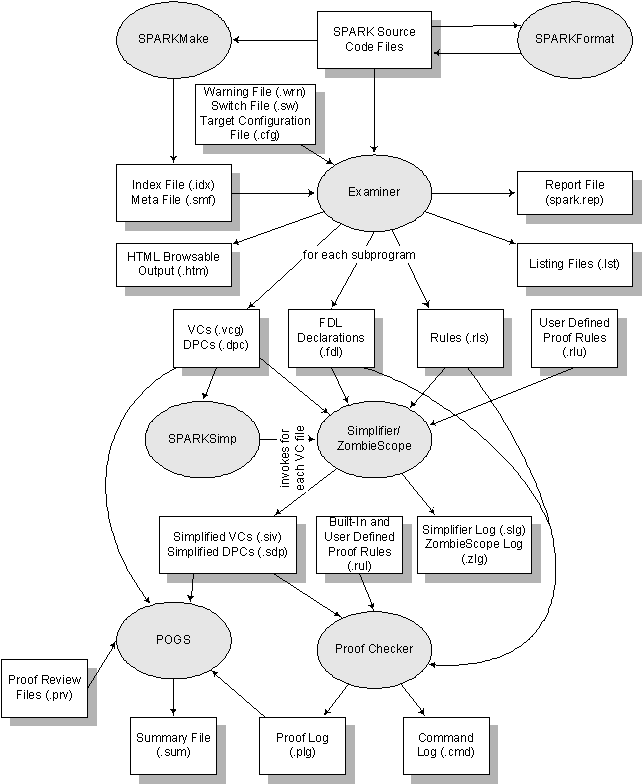
\includegraphics[height=0.6\textheight]{figures/spark-tools.png}    	
    \end{center}
    \caption{Relationship of the Examiner and Proof Tools.\protect\footnotemark}
    \label{figure:spark-tools}
\end{figure}
\footnotetext{http://docs.adacore.com/sparkdocs\-docs/Examiner\_UM.htm}

\newpage

SPARK includes a development and verification tool-set with the following components:
\begin{itemize}
	\item SPARKMake - generates index file (.idx) and meta file (.smf)
	\item Examiner - checks syntax, generates Verification Conditions (VCs) and Dead Path Conjectures (DPCs), and discharges (proves) some of them (some might be impossible to discharge)
	\item Simplifier - simplifies VCs (not discharged by Examiner) and tries to discharge them after simplification process in similar fashion like Examiner
	\item ZombieScope - finds dead paths
	\item ViCToR - translates VCs and DPCs to format acceptable by SMT solver and proves correctness using specified SMT solver
	\item SPARKSimp - runs Simplifier or/and ZombieScope
	\item POGS - produces verification report
	\item Proof Checker - discharges VCs or DPCs not discharged by Examiner and Simplifier by carrying out tool-assisted manual proof steps
\end{itemize}

Relationships between tools and verification flow is presented in the Figure \ref{figure:spark-tools}. SPARK proof tools use FDL as the modeling language. 



\subsection{SPARK Examiner}
\label{background:sparkverification:examiner}

The main SPARK verification tool is Examiner. It supports several levels of analysis:
\begin{itemize}
	\item checking of SPARK language syntactic and static semantic rules
	\item data flow analysis
	\item data and information flow analysis
	\item formal program verification via generation of verification conditions
	\item proof of absence of run-time errors
	\item dead path analysis
\end{itemize}

There is an option to make the Examiner perform syntax checks only. Using this option on a source file does not require access to any other units on which the file depends, so files can be syntax checked on an individual basis. This allows any syntax errors to be corrected before the file is included in a complex examination \cite{Examiner:Online}.

Examiner can perform data and information analysis of Ravenscar programs in exactly the same manner as for sequential programs \cite{Ravenscar:Online}. Unfortunately it does not allow protected objects in proof annotations (pre- and post-conditions) as mentioned in Section \ref{background:spark:ravenscar}.

When some parts of the system are written in full Ada (with non-valid SPARK constructs), then Examiner returns error. Ada parts can be excluded from Examiner analysis using \lstinline{--# hide} annotation. Then, only a warning is returned by Examiner: \lstinline{10 - The body of subprogram Main is hidden - hidden text is ignored by the Examiner}.

Examiner use SPARK index file (.idx) - generated by \lstinline{SPARKMake} tool -  to locate files necessary for verification \cite{Barnes:Book}.

Examiner can be used with the \lstinline{spark} command and appropriate flags described in Examiner Manual \cite{Examiner:Online}.

%http://docs.adacore.com/sparkdocs-docs/SPARK_GPS.htm

To use Examiner in GNAT Programming Studio:
\begin{itemize}
	\item Run SPARK Make: right click on project / SPARK / SPARK Make (Figure \ref{figure:sparkmake})
	\item Set SPARK index file (to spark.idx generated by SPARKMake) (Figure \ref{figure:examinerproperties})
	\item (optionally) set configuration file (e.g. Standard.ads)
	\item Choose appropriate version of SPARK (95 or 2005)
	\item Choose mode: Sequential (for single tasking programs) or Ravenscar (for multitasking programs)
\end{itemize}

\begin{figure}[ht]%t=top, b=bottom, h=here
    \begin{center}
    	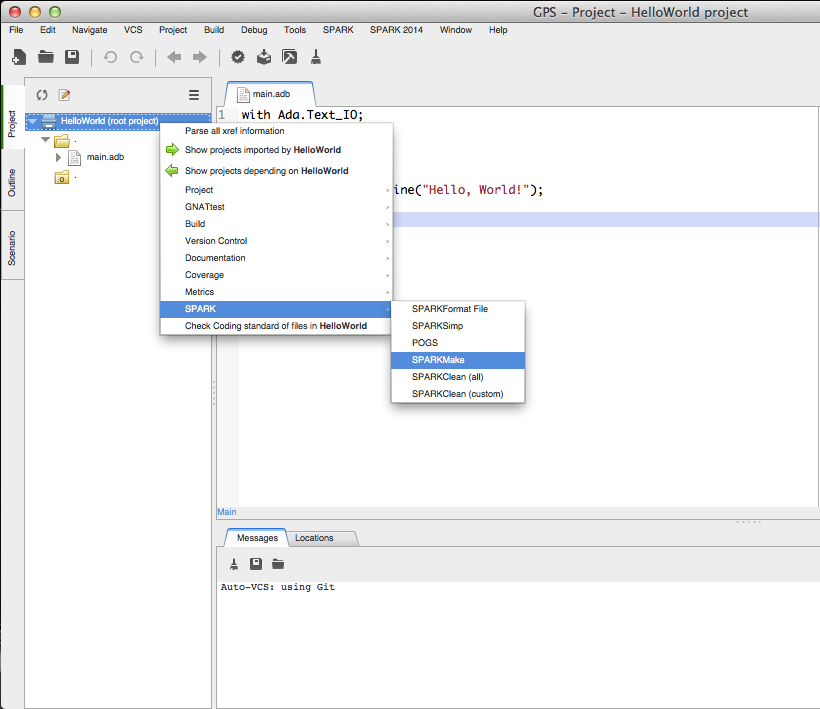
\includegraphics[width=0.55\textwidth]{figures/SPARKMake.png}    	
    \end{center}
    \caption{Run SPARK Make}
    \label{figure:sparkmake}
\end{figure}

\begin{figure}[ht]%t=top, b=bottom, h=here
    \begin{center}
    	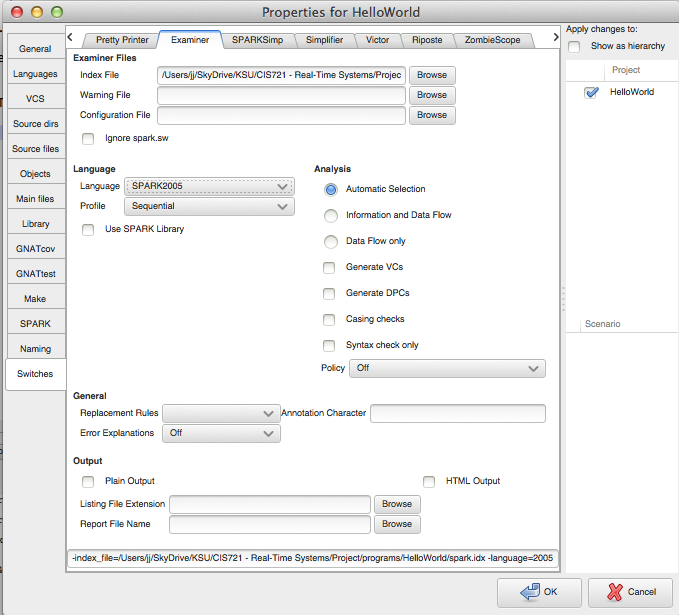
\includegraphics[width=0.6\textwidth]{figures/Properties-Switches-Examiner.png}    	
    \end{center}
    \caption{Examiner Properties}
    \label{figure:examinerproperties}
\end{figure}

To generate verification conditions (VCs), the \lstinline{-vcg} switch has to be used. It can be set in GNAT Programming Studio (Project / Edit project properties / Switches / Examiner / Generate VCs).
In addition to verification conditions, Examiner can check dead path conjectures (DPCs), i.e. paths through the code that can never be executed regardless of input. To generate dead path conjectures, the \lstinline{-dpc} switch has to be used. It can be also set in GNAT Programming Studio (Project / Edit project properties / Switches / Examiner / Generate DPCs).

Examiner has been used to check syntax and semantics during PCA Pump Prototype development and in verification process described in Chapter \ref{verification}.


\subsubsection{Flow analysis}
\label{background:sparkverification:examiner:flowanalysis}
%http://www.cs.swan.ac.uk/~csetzer/lectures/critsys/09/critsysfinal2.pdf
There are two types of flow analysis:
\begin{itemize} \itemsep1pt \parskip0pt \parsep0pt
	\item Data flow analysis:
	\begin{itemize} \itemsep1pt \parskip0pt \parsep0pt
		\item Checks input/output behavior of parameters and variables.
		\item Checks initialization of variables.
		\item Checks that changed and imported variables are used later (possibly as output variables).
	\end{itemize}
	\item Information flow analysis - verifies interdependencies between variables.
\end{itemize}

In data flow analysis, Examiner checks if input parameters are not modified, but used at least once (in at least one branch of program). In the same factor, output parameters cannot be read (before initialization) and has to be initialized (in all branches of program). Input/output parameters has to be both read and write (changed). In similar way, Examiner verify the global variables (specified in annotations). Functions can use only input parameters and can only read global variables. Therefore functions do not have side effects. 

Global variables defined in package body (thus private) has to be declared by \lstinline{--# own} annotation in package specification. If variable is also initialized, \lstinline{--# initializes} annotation has to be used. In Ada, to use package in another package, \lstinline{with} clause has to be used. In SPARK Ada, additionally \lstinline{--# inherits} annotation has to be specified.

In information flow analysis, dependencies between variables are analyzed. These dependencies are specified by \lstinline{--# derives} annotation.


\subsubsection{Verification conditions}
\label{background:sparkverification:examiner:vc}

Verification conditions is a set of generated hypothesis, if proven to be true can be concluded that they hold. To generate verification conditions, two kinds of annotations are relevant for Examiner:
\begin{itemize}
	\item preconditions: \lstinline{--# pre}
	\item postconditions: \lstinline{--# post}
\end{itemize}

The notions of pre- and postconditions are based on Hoare logic \cite{HoareLogic:Paper}. More precisely, in the Hoare triple below: 

\begin{equation} \label{eq:hoare_triple}
	\{P\} C \{Q\}
\end{equation}

\lstinline{C} is a program that starts in a state satisfying precondition \lstinline{P}. Program terminates in stat satisfying postcondition \lstinline{Q}. Thus \lstinline{P} and \lstinline{Q} are assertions, and \lstinline{C} is a command (action) performed between them.

Additionally, assertions (\lstinline{--# assert}) and checks (\lstinline{--# check}) can be specified in procedure body. Then additional verification conditions are generated.

SPARK functions do not have side effects (as stated in \ref{background:sparkverification:examiner:flowanalysis}), thus only preconditions are relevant. However, there is annotation \lstinline{--# return}, which specifies function return value.

Verification Conditions (VCs) are generated depending on commands appearing in the subprogram along path segments. VC generation is performed backwards, in other words: we start from post-conditions and consider what must holds before. Flow analysis is well described in chapter 11 of \cite{Barnes:Book}.

If preconditions are not present, then the formula expresses that the post-condition holds always.



\subsection{SPARK Simplifier}
\label{background:sparkverification:simplifier}

Simplifier, simplifies Verification Conditions (VCs) generated by Examiner. It can also discharge (prove correctness) of those VCs, which are not proved by Examiner \cite{Simplifier:Online}. It takes as input \lstinline{.vcg} files, \lstinline{.fdl} files for its data declarations and - if available - proof-rule files (\lstinline{.rls}, \lstinline{.rlu}). Then it generates \lstinline{.siv} files (simplified VCs) and \lstinline{.slg} files (which contain details about simplification that has been made).

SPARK Simplifier has been used in verification process described in Chapter \ref{verification}.



\subsection{ZombieScope}
\label{background:sparkverification:zombiescope}

ZombieScope is a SPARK tool that analyze SPARK code to find dead paths, i.e. paths through the code that can never be executed. A program that contains dead paths may not necessarily be incorrect, but a dead path is an indication of a potential code issue.

ZombieScope reads \lstinline{.dpc} files generated by the Examiner. In order to generate dead path conjectures, \lstinline{-dpc} flag has to be used or 'Generate DPCs' option has to be checked in Examiner options, in GPS. It reads also \lstinline{.fdl} files for its data declarations and the \lstinline{.rls} file for proof-rules if present. ZombieScope generates two output files: \lstinline{.sdp} file (dead path summary) and \lstinline{.zlg} file (details about underlying contradiction search performed). ZombieScope is invoked by SPARKSimp by default and the summary file generated by POGS includes information about the dead path analysis.

ZombieScope has been used for dead paths analysis in verification process described in Chapter \ref{verification}.



\subsection{ViCToR}
\label{background:sparkverification:victor}

ViCToR is a tool to translate Verification Conditions (VCs), generated by the Examiner, into SMT-LIB (file format used to communicate with SMT solvers) \cite{Victor:Online}. SMT (Satisfiability Modulo Theories) solver is a tool for verification and proving the correctness of programs. ViCToR is integrated with SPARKSimp and POGS. To invoke ViCToR from SPARKSimp, flag \lstinline{-victor} has to be used.

ViCToR has been used in verification process described in Chapter \ref{verification}.



\subsection{Proof Checker}
\label{background:sparkverification:proofchecker}

% Barnes' book: 12.12
Proof Checker is advanced verification tool, which require considerable experience in verification of SPARK programs. It is interactive program, which enables the user to direct the Checker to explore the use of various strategies and rules on the condition to be proved. Proof Checker can keep a log of the progress of a proof in \lstinline{plg} file. It also records the proof steps applied in a \lstinline{.cmd} file. More details about Proof Checker can be found in chapter 12 of \cite{Barnes:Book}.

Proof Checker was not used in this thesis. Instead Bakar Kiasan (see section \ref{background:sparkverification:sireum}) has been used.



\subsection{SPARKSimp Utility}
\label{background:sparkverification:sparksimp}
SPARKSimp is a simple "make" style tool for the SPARK analysis tools. Currently, it supports the Simplifier, ZombieScope and ViCToR. It applies the Simplifier (and ViCToR, if requested) to all \lstinline{.vcg} files and ZombieScope to all \lstinline{.dpc} files that it finds in a directory tree \cite{SPARKSimp:Online}.

SPARKSimp has been used to invoke Simplifier, ZombieScope and ViCToR in verification performed in this thesis (see Chapter \ref{verification}).



\subsection{Proof Obligation Summarizer (POGS)}
\label{background:sparkverification:pogs}

The Proof ObliGation Summarizer tool (POGS) reads and understands the structure of the verification conditions (\lstinline{.vcg} files), their simplified version (\lstinline{.siv} files), and dead path conjectures (\lstinline{.dpc} files). It reports the status of proofs and dead path analyses in a human-readable, text form \cite{POGS:Online}.

POGS has been used to generate reports for verification performed in this thesis (see Chapter \ref{verification}). 



\subsection{AUnit}
\label{background:sparkverification:aunit}

AUnit is a unit test framework for the Ada language. It can be also applied to test SPARK Ada programs. It was inspired by Java JUnit (created by Kent Beck, Erich Gamma) and C++ CppUnit (created by M. Feathers, J. Lacoste, E. Sommerlade, B. Lepilleur, B. Bakker, S. Robbins) unit test frameworks \cite{AUnitCookbook:Online}. Similar to these related frameworks, it enables simple test cases execution, fixtures, suites, and provides reporting \cite{AUnitTutorials:Online}. 

GNAT Programming Studio can generate test cases skeleton for all subprograms. It can be generated using Tools -> GNATtest -> Generate unit test setup. This generator creates a new project with AUnit tests. The project for which tests are generated is referenced in new generated test project. In order to run tests, the test project has to be opened in GNAT Programming Studio. The project is created in \lstinline{[project_dir]/gnattest/harness/test_[proj_name].gpr}. It generates an empty (not implemented) test for each subprogram in project. To add/edit/remove tests or rename names, three files have to be edited:

\begin{itemize}
    \item \lstinline{[some_package]-test_data-tests.ads}
    \item \lstinline{[some_package]-test_data-tests.adb}
    \item \lstinline{[some_package]-test_data-tests-suite.adb}
\end{itemize}

Each test has to be declared in \lstinline{[some_package]-test_data-tests.ads} and implemented in \lstinline{[some_package]-test_data-tests.adb}. Then, it has to be added to test suite in \lstinline{[some_package]-test_data-tests-suite.adb} file.

Tests can be also created manually. Then, the AUnit distribution has to be referenced in project file, and all test cases (and suits) have to be implemented by hand.

AUnit has been used to create unit test for isolated module of created PCA Pump Prototype (see Section \ref{verification:aunit}).



\subsection{Sireum Bakar}
\label{background:sparkverification:sireum}

Sireum\footnote{http://www.sireum.org/} is a long-term research project conducted by SAnToS Laboratory at Kansas State University. Its goal is to develop an over-arching software analysis platform that incorporates various static analysis techniques such as a data-flow framework, model checking, symbolic execution, abstract interpretation, and deductive reasoning techniques (e.g., using weakest precondition calculation). It can be used to build various kinds of software static analyzers for different kinds of properties. 

It uses the Pilar language \cite{Pilar:Paper} as an intermediate representation. Any language which can be translated to Pilar can be analyzed by Sireum. For now, there are translators for SPARK and Java.

Bakar is a toolset for analyzing SPARK Ada programs (Bakar means "spark" in Indonesian). Sireum Bakar currently includes:
\begin{itemize}
	\item Kiasan - functional behaviors verification tool
	\item Alir - information flow analysis tool	
\end{itemize}

The Sireum distribution is available for Windows (32-bit, 64-bit), Linux (32-bit, 64-bit) and MacOS (64-bit). It can be downloaded from \lstinline{http://www.sireum.org/}.


\subsubsection{Bakar Kiasan}

Bakar Kiasan \cite{Kiasan:Paper} is a fully automated tool for verifying functional behaviors of SPARK programs specified as software contracts. Kiasan use symbolic execution technique (Kiasan means "symbolic" in Indonesian). It provides various helpful feedback including generation of counter example for contract refutation, test cases for an evidence of contract satisfaction, verification reports, visual graphs illustrating pre/post states of SPARK procedures/functions, etc. It is much easier to understand than, e.g., analysis of \lstinline{.vcg} files generated by SPARK Examiner.

There exists a Kiasan Plug-in for GNAT Programming Studio (GPS). Version 1, for GPS 5, supports SPARK 2005. Version 2, for GPS 6, which supports SPARK 2014, is under development. Both plug-ins are created by author of this thesis in Python and PyGTK. There is also plug-in for Eclipse, but only for SPARK 2005 programs.

Bakar Kiasan does not support the Ravenscar profile. Thus, it can be used only for sequential programs verification. Figure \ref{figure:kiasan-sample} presents sample Kiasan analysis result. The Kiasan window in GPS has two parts: (i) a list of units (packages and subprograms), and (ii) analysis cases with pre- and post states. Every unit has the following associated statistics:
\begin{itemize}
	\item T\# - Test cases (expected behavior),
	\item E\# - Exception cases (unexpected behavior),
	\item Instruction coverage - amount of code that will be executed in execution paths generated by Kiasan analysis,
	\item Branch coverage - number of branches discovered by Kiasan analysis (0\% branch coverage in the case of 100\% instruction coverage means that there are no branches in the analyzed unit), and
	\item Time in which analysis was performed.
\end{itemize}

After double clicking on some unit, code that is executed during execution of this unit is highlighted. Additionally below the list of units, there is a combo box which contains all test cases associated with the selected (by double clicking) unit. Once some case is selected, code coverage equivalent to this test case is highlighted. Additionally, below the combo box, there are generated execution cases - one for each execution path. The pre-state is listed on the left hand side while the post state is listed on the right hand side. Variables with red font color, in the post-state, are those that are changed as the result of unit execution. Newly created variables (during unit execution) are marked in blue, but there are no such variables in the example presented in Figure \ref{figure:kiasan-sample}.

\begin{figure}[ht]%t=top, b=bottom, h=here
    \begin{center}
    	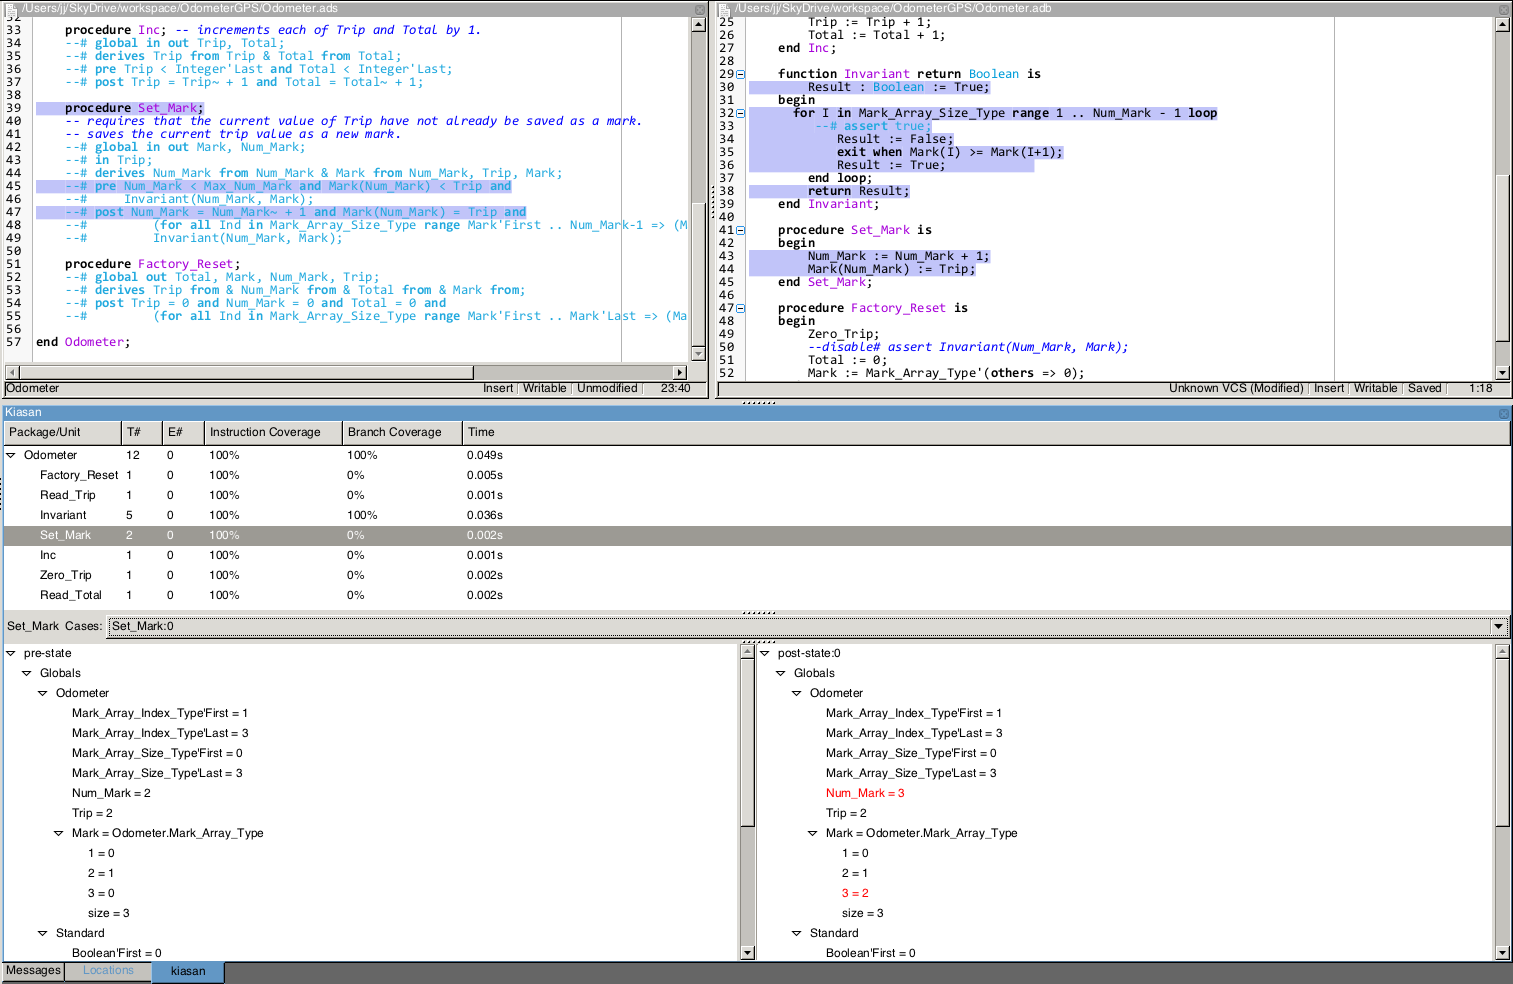
\includegraphics[width=0.9\textwidth]{figures/kiasan-sample.png}    	
    \end{center}
    \caption{Bakar Kiasan report}
    \label{figure:kiasan-sample}
\end{figure}

Bakar Kiasan is useful especially for solving verification issues. It can generate counter examples that give developers greater intuition about problems in the code.

Bakar Kiasan has been used in verification of PCA Pump module (see Section \ref{verification:pcapump:monitoring}).



\subsubsection{Bakar Alir}
Alir is an information flow analysis tool for reasoning about SPARK's derive clauses/information flow (Alir means "flow" in Indonesian). Alir visualizes information flows to ease engineers in understanding information dependencies crucial for specifying and verifying SPARK's derive clauses. It provides various configurable intra-procedural and inter-procedural analyses. The inter-procedural analyses are control flow analysis, reaching definition analysis and data dependence analysis. The inter-procedural analyses in Alir include building the System Dependence Graph (SDG), slicing and chopping on SDG \cite{Hari:Thesis}.

Bakar Alir has not been used in this thesis, but can potentially be used in the future, to enrich verification process.


\subsection{GNATprove}
\label{background:sparkverification:gnatprove}
% http://docs.adacore.com/spark2014-docs/html/ug/gnatprove.html
% https://github.com/openETCS/model-evaluation/wiki/Gnatprove-description

GNATprove\footnote{http://www.open-do.org/projects/hi-lite/gnatprove/} is a formal verification tool for SPARK 2014 programs, whose input is automatically constructed using GNAT compiler as a front-end. GNATprove interprets SPARK Ada annotations exactly like they are interpreted at run time during tests. It can prove that subprograms respect their contracts, expressed as preconditions and postconditions in the syntax of Ada 2012. The tool automatically discovers the subset of subprograms which can be formally analyzed. GNATprove is currently available for Linux x86, Windows x86 and Linux x86-64.

GNATprove consists of two distinct analyses, flow analysis and proof. Flow analysis checks the correctness of aspects related to data flow (\lstinline{Global}, \lstinline{Depends}, \lstinline{Abstract_State}, \lstinline{Initializes}, and refinement versions of these), and verifies the initialization of variables. Proof verifies the absence of runtime errors and the correctness of assertions such as \lstinline{Pre} and \lstinline{Post} aspects. Using the switch \lstinline{--mode=<mode>}, whose possible values are \lstinline{flow}, \lstinline{prove} and \lstinline{all}, only one or both of these analyses can be performed (\lstinline{all} is the default) \cite{Spark2014userGuide:Online}. GNATprove use Alt-Ergo prover for verification.

GNATprove has been used to verify isolated module of created PCA Pump Prototype, which has been translated to SPARK 2014 (see Section \ref{verification:gnatprove}).



\section{AADL/BLESS to SPARK Ada code generation}
\label{background:codegen}

The ultimate goal of the long term research of which this thesis is part is to build an AADL (with BLESS) to SPARK Ada translation. AADL has been used to prototype and fully develop embedded systems for the past 5-7 years \cite{PrototypyingAadl:Paper}. Related work in code generation from AADL, but for Java programming language has been done in \cite{MAP:Paper}. There are also already existing tools, which performs code generation based on AADL:
\begin{itemize} %\itemsep1pt \parskip0pt \parsep0pt
	\item Ocarina
	\item Ramses
\end{itemize}



\subsection{Ocarina}
\label{background:codegen:ocarina}

Ocarina \cite{Ocarina:Paper} is a tool suite that contains plug-ins for code generation, model checking and analysis. The code generation plug-in generates code from an AADL architecture model to an Ada or C application running on top of PolyORB framework. In this context, PolyORB acts as both the distribution middleware and execution runtime on all targets supported by PolyORB. Ocarina is written in Ada.

There is plug-in for OSATE (see Section \ref{background:aadl:osate}) that supports code generation. Example AADL models, suitable for being an input of Ocarina are available on github repository: \lstinline{https://github.com/yoogx/polyorb-hi-ada/tree/master/examples/aadlv2}.

Since mid-2009, Telecom ParisTech is no longer involved in Ocarina, and is developing another AADL tool-chain, based on Eclipse, codenamed RAMSES \cite{RAMSES:Paper}.

Ocarina has been used as inspirational tool for code generation from AADL models.  



\subsection{RAMSES}
\label{background:codegen:ramses}
% http://penelope.enst.fr/aadl/wiki/Projects
% http://www.aadl.info/aadl/downloads/committee/feb2013/presentations/RAMSES_status_2013_06_02_format.pdf

RAMSES (Refinement of AADL Models for Synthesis of Embedded Systems) \cite{RAMSES:Paper} is a model transformation and code generation tool written in Java. Code generation module produces C code, but does not generate Ada. The approach for code generation is to transform AADL models using a rule-based transformation framework and generate code from transformed (simplified) models. Simplified AADL models contain behavior annex subclauses. RAMSES can be used as OSATE plug-in or standalone application.

RAMSES was initial point of interest, because of its code generation module. However, it has not been used due to its limitation to generate C code only.

